\section{AJ-RNN}
% TODO paper overview

\subsection{Adverarial learning}

\subsection{Data preparation}
- 

\subsection{Model}
- model overview

\begin{figure}[!htbp]
  \centering
  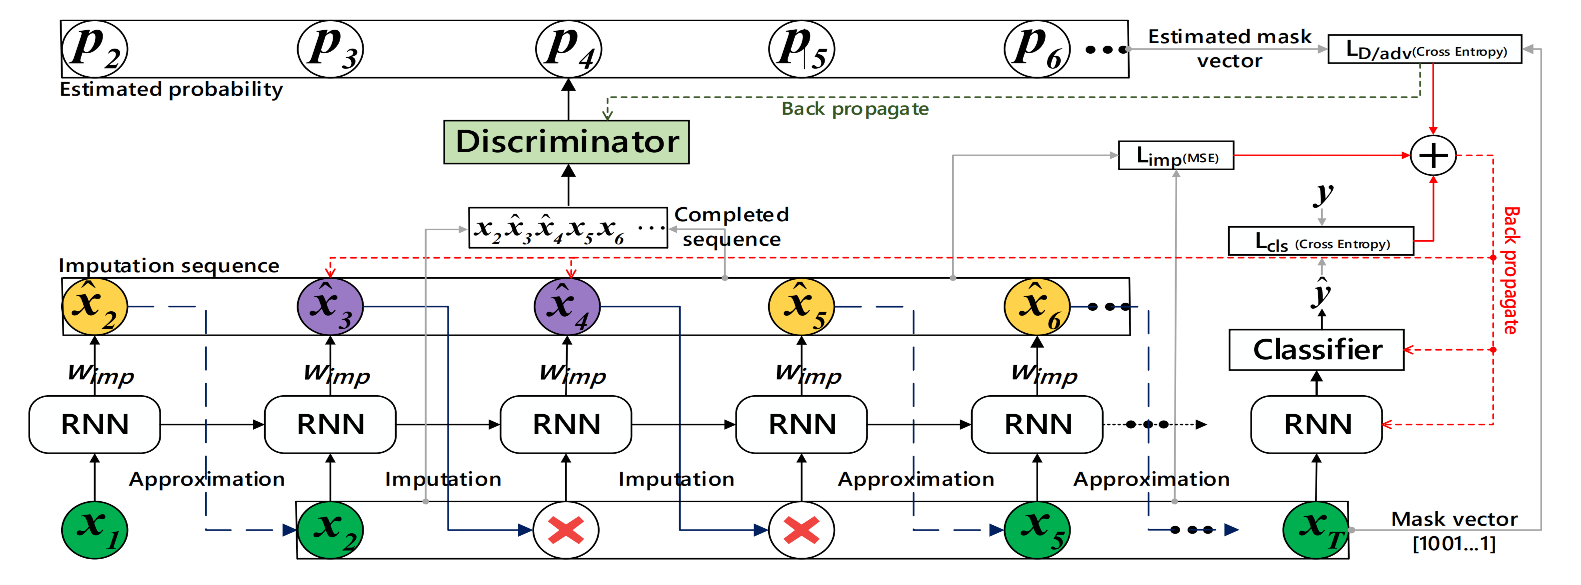
\includegraphics[width=1\textwidth]{ajrnn}
  \caption{The proposed AJ-RNN framework. We use green units to denote revealed inputs, yellow for the output of approximated values, purple for
  the imputed values and a red “X” for missing inputs. Dashed links are for approximation training and solid ones are for imputation. The discriminator
  receives a completed vector composed of revealed and imputed values as input, which provides a one-to-one supervisory signal for imputed values
  $\hat{x_3}$ and $\hat{x_4}$.    \cite{ajrnn}}
  \label{tab:AJRNNrchitecture}
\end{figure}

\subsection{Experimental results}
- implemented in tensoflow 2.0 (modularized)\\
-- made sure that acucracy was the same as in the paper\\
-- added support for multivariate time series\\
- experimented with different configurations 

\begin{paragraph}{Cell type}
learning rate = 0.001, batch size = 256, G-epochs = 1

\begin{table}[!htbp]
  \centering
  \begin{tabular}{cccr} 
      Cell type & Cell size & Dropout & Overall Accuracy\\[0.2cm] 
      \hline \\[-0.2cm] 
      GRU   &   64  & 0.2 &  $84.10 \pm 3.72$\\
      GRU   &   64  & 0.4 &  $81.75 \pm 4.18$\\
      GRU   &   64  & 0.6 &  $79.70 \pm 4.92$\\
      GRU   &   64  & 0.8 &  $82.78 \pm 4.26$\\[0.05cm] \hline \\[-0.25cm]
      GRU   &   128 & 0.2 &  $78.58 \pm 4.17$\\
      GRU   &   128 & 0.4 &  $80.84 \pm 0.00$\\
      GRU   &   128 & 0.6 &  $70.07 \pm 9.58$\\
      GRU   &   128 & 0.8 &  $81.03 \pm 4.66$\\[0.05cm] \hline \\[-0.25cm]
      GRU   &   256 & 0.2 &  $80.49 \pm 8.77$\\
      GRU   &   256 & 0.4 &  $75.25 \pm 1.88$\\
      GRU   &   256 & 0.6 &  $75.97 \pm 1.43$\\
      GRU   &   256 & 0.8 &  $77.34 \pm 1.74$\\[0.05cm] \hline \\[-0.25cm]
      LSTM  &   64  & 0.2 &  $79.41 \pm 1.76$\\
      LSTM  &   64  & 0.4 &  $84.92 \pm 3.69$\\
      LSTM  &   64  & 0.6 &  $81.16 \pm 4.99$\\
      LSTM  &   64  & 0.8 &  $0.00 \pm 0.00$\\[0.05cm] \hline \\[-0.25cm]
      LSTM  &   128 & 0.2 &  $84.89 \pm 3.00$\\
      LSTM  &   128 & 0.4 &  $85.08 \pm 0.35$\\
      LSTM  &   128 & 0.6 &  $83.24 \pm 4.29$\\
      LSTM  &   128 & 0.8 &  $82.39 \pm 1.99$\\[0.05cm] \hline \\[-0.25cm]
      LSTM  &   256 & 0.2 &  $74.18 \pm 3.44$\\
      LSTM  &   256 & 0.4 &  $67.15 \pm 15.02$\\
      LSTM  &   256 & 0.6 &  $71.36 \pm 22.56$\\
      LSTM  &   256 & 0.8 &  $85.37 \pm 2.37$\\ 
      
  \end{tabular}
  \caption{Overall accuracy with different configurations for Cell type, Cell size and Dropout}
  \label{tab:AJRNNCellTypeResults}
\end{table}

\end{paragraph}

\begin{table}[!htbp]
  \centering
  \begin{tabular}{cccr} 
      Batch size & Learnig rate & Dropout & Overall Accuracy\\[0.2cm] 
      \hline \\[-0.2cm]
      256 &   1e-03 &   0.0 & $86.13 \pm 0.00$\\
      256 &   1e-03 &   0.2 & $78.58 \pm 4.17$\\
      256 &   1e-03 &   0.4 & $81.05 \pm 4.39$\\
      256 &   1e-03 &   0.6 & $73.03 \pm 9.81$\\
      256 &   1e-03 &   0.8 & $81.03 \pm 4.66$\\[0.05cm] \hline \\[-0.25cm]

      256 &   1e-04 &   0.4 & $80.00 \pm 2.91$\\
      256 &   1e-04 &   0.6 & $85.46 \pm 2.01$\\
      256 &   1e-04 &   0.8 & $83.88 \pm 4.33$\\[0.05cm] \hline \\[-0.25cm]

      32  &   1e-03 &   0.2 & $32.45 \pm 4.42$\\
      32  &   1e-03 &   0.6 & $28.21 \pm 6.00$\\
      32  &   1e-03 &   0.8 & $23.07 \pm 1.05$\\
      32  &   1e-04 &   0.0 & $30.26 \pm 0.00$\\[0.05cm] \hline \\[-0.25cm]

      32  &   1e-04 &   0.2 & $39.49 \pm 5.91$\\
      32  &   1e-04 &   0.4 & $28.93 \pm 0.00$\\
      32  &   1e-04 &   0.6 & $25.64 \pm 0.00$\\
      32  &   1e-04 &   0.8 & $32.97 \pm 0.00$\\[0.05cm] \hline \\[-0.25cm]

      32  &   1e-05 &   0.8 & $67.12 \pm 0.00$\\[0.05cm] \hline \\[-0.25cm]
      32  &   1e-08 &   0.0 & $73.32 \pm 2.83$
  \end{tabular}
  \caption{Overall accuracy with different configurations for Batch size, Learning rate and Dropout}
  \label{tab:AJRNNBatchSizeResults}
\end{table}








- learnig rate\\
- batch size \\
- G-epochs

\subsection{Light AJ-RNN}
- model overview\\
- baseline